\documentclass[10pt,a4paper]{report}
\usepackage[utf8]{inputenc}
\usepackage{amsmath,mathtools}
\usepackage{amsfonts}
\usepackage{amssymb}
\usepackage{graphicx}
\usepackage{hyperref}
\usepackage{bm}
\usepackage{gensymb}
\usepackage{listings} 	
\usepackage[left=2cm,right=2cm,top=2cm,bottom=2cm]{geometry}
\setlength\parindent{0pt}
\graphicspath{{./images/}}
\newcommand{\legendre}[2]{(\frac{#1}{#2})}


\usepackage[english]{babel}
 
\usepackage{amsthm}
 
\newtheorem*{prop}{Proposition}
\newtheorem*{theorem}{Theorem}
\begin{document}


\textbf{CATAM Part II - 15.10 - The Continued Fraction Method for
Factorization}
\thispagestyle{empty}

\newpage

\subsection*{Introduction}

\subsection*{Question 1}
We implement the B smoothness test as $B\_smooth(B,N)$, which either returns a list of divisors, or False. To estimate the probability a d-digit integer, ie an integer in range $[10^{d-1},10^d-1]$, is B-smooth with the given set of primes $\l 50$, we test all integers up to $10^6$ explicitly, then take a random sample of size $900000 = | [10^{6-1},10^6-1] |$ for higher d. The probabilities we get are:

\begin{table}[h]
\centering
\begin{tabular}{|l|l|l|l|l|l|l|l|l|l|l|}
\hline
k                     & 1 & 2    & 3    & 4    & 5     & 6     & 7      & 8      & 9      & 10     \\ \hline
estimated probability & 1 & .888 & .488 & .215 & .0797 & .0258 & .00743 & .00205 & .00049 & .00011 \\ \hline
\end{tabular}
\caption{Estimated probability a d digit number is B-smooth}
\label{tab:my-table}
\end{table}

\begin{figure}[h]
\centering
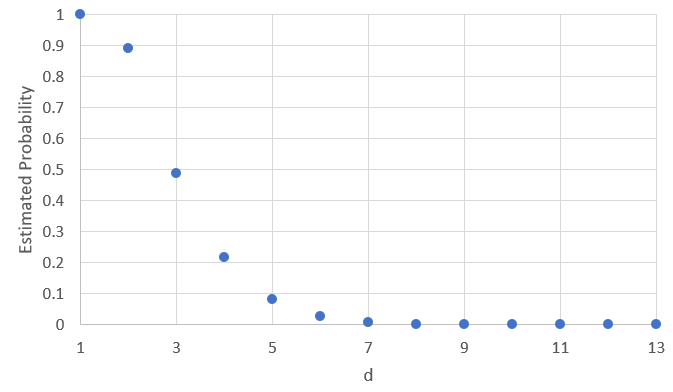
\includegraphics[width=10cm]{q1graph.png}
\caption{Graph of \ref{tab:my-table}}
\end{figure}

The function written checks divisibility of N by p by calculating $N \mod p$. For very large N we could handle this if required by iterating over the digits of $N$. If $N=a_oa_1a_2\dots a_n$ written in decimal, we can initialise $result=0$ and iterate $result=result\times10+a_k\pmod p$ for $k=0,1\dots n$.	

\subsection*{Question 2}

\begin{prop}
If $x =\sqrt{N}$ for some positive integer $N$ then each $x_n$ may be written in the form $(r +\sqrt{N})/s$ with $r, s$ integers and $s \mid (r^
2 - N)$.
\end{prop}

\begin{proof}

Proceed by induction. For the base case $n=0$ we have $x_0=x=\sqrt{N}$ so $r=0$, $s=1$ and so $s \mid (r^2 - N)$. For the inductive step, assume $x_n$ may be written as $(r +\sqrt{N})/s$ with $r,s$ integers satisfying $s \mid (r^2 - N)$. Then compute $x_{n+1}$. 

\begin{align*}
x_{n+1} &= \frac{1}{x_n-a_n}\\
		&= \frac{1}{\frac{r+\sqrt{N}}{s}-a_n}\\
		&= \frac{s}{\sqrt{N}+(r-a_ns)}\\
		&= \frac{s(\sqrt{N}-r+a_ns)}{N-r^2-a_n^2s^2+2ra_ns}\\
		&= \frac{\sqrt{N}+(a_ns-r)}{\frac{N-r^2}{s}-a_n^2s+2ra_n}\\
\end{align*}

so we have 

\begin{align*}
r' &= a_ns-r\\
s'	&= \frac{N-r^2}{s}-a_n^2s+2ra_n\\
\end{align*}

and thus 

\begin{align*}
r'^2-N &= a_n^2s^2+r^2-2a_nsr-N\\
	&= s(\frac{N-r^2}{s}-a_n^2s+2ra_n)\\
	&= ss'\\
\end{align*}

ie $s' \mid (r'^2 - N)$ as required.

\end{proof}

This proposition allows us to store $x_n$ without worry of rounding errors. From IIC Number Theory, we know the sequence of partial quotients is of form $[a_0;\overline{a_1,\dots,a_n}]$, and in particular is  eventually periodic. The function $sqrt\_cont\_frac(N,k)$ is our implementation, with k giving a maximum number of partial quotients to return, in case of a very long period. The partial quotients for $\sqrt{N}$, N up to 50 are generated and printed by $q2i()$, with the integers after the colon being the repeated period:

\begin{lstlisting}[breaklines]
0 ) 0 
1 ) 1 
2 ) 1 : 2
3 ) 1 : 1, 2
4 ) 2 
5 ) 2 : 4
6 ) 2 : 2, 4
7 ) 2 : 1, 1, 1, 4
8 ) 2 : 1, 4
9 ) 3 
10) 3 : 6
11) 3 : 3, 6
12) 3 : 2, 6
13) 3 : 1, 1, 1, 1, 6
14) 3 : 1, 2, 1, 6
15) 3 : 1, 6
16) 4 
17) 4 : 8
18) 4 : 4, 8
19) 4 : 2, 1, 3, 1, 2, 8
20) 4 : 2, 8
21) 4 : 1, 1, 2, 1, 1, 8
22) 4 : 1, 2, 4, 2, 1, 8
23) 4 : 1, 3, 1, 8
24) 4 : 1, 8
25) 5 
26) 5 : 10
27) 5 : 5, 10
28) 5 : 3, 2, 3, 10
29) 5 : 2, 1, 1, 2, 10
30) 5 : 2, 10
31) 5 : 1, 1, 3, 5, 3, 1, 1, 10
32) 5 : 1, 1, 1, 10
33) 5 : 1, 2, 1, 10
34) 5 : 1, 4, 1, 10
35) 5 : 1, 10
36) 6 
37) 6 : 12
38) 6 : 6, 12
39) 6 : 4, 12
40) 6 : 3, 12
41) 6 : 2, 2, 12
42) 6 : 2, 12
43) 6 : 1, 1, 3, 1, 5, 1, 3, 1, 1, 12
44) 6 : 1, 1, 1, 2, 1, 1, 1, 12
45) 6 : 1, 2, 2, 2, 1, 12
46) 6 : 1, 3, 1, 1, 2, 6, 2, 1, 1, 3, 1, 12
47) 6 : 1, 5, 1, 12
48) 6 : 1, 12
49) 7 
50) 7 : 14
\end{lstlisting}


The following claims have all been verified numerically up to N=$10^6$, by $q2ii()$. In fact they are all true, but we will omit proofs here, and instead link to some references.\\

We first observe they all have fairly short periods, less than N say. See \footnote{\url{http://web.math.princeton.edu/mathlab/jr02fall/Periodicity/mariusjp.pdf}, Corollary 2.1}\\

Secondly, we see that the partial quotients take form $\sqrt{N} = [a_0; \overline{a_1, a_2, \dots, a_{l-1}, 2a_0}]$ with $a_1, a_2, \dots, a_{l-1}$ palindromic\footnote{This is a well known theorem. See for example Ex 12.2.13 in Rosen, "Elementary Number Theory". The text provides a proof at the back.}.  	\\

We further have that  $a_1, a_2, \dots, a_{l-1} < \sqrt{N}$, true up to $10^5$. max(r) $\approx\sqrt{N}$, r satisfies $r<\sqrt{N}$, and s satisfies $s<2\sqrt{N}$. See \footnote{\url{https://math.stackexchange.com/questions/2838367/size-of-partial-quotients-in-continued-fraction-expansion-of-sqrtn}}. This can be shown by carefully handling inequalities in the above induction.

\subsection*{Question 3}

The function $q3()$, using $convergents()$ produces the following data. I've included the length of the period in square brackets for later reference.

\begin{lstlisting}[breaklines]
 3 [2]) -2, 1, -2, 1, -2, 1, -2, 1, -2, 1
 5 [1]) -1, 1, -1, 1, -1, 1, -1, 1, -1, 1
 7 [4]) -3, 2, -3, 1, -3, 2, -3, 1, -3, 2
12 [2]) -3, 1, -3, 1, -3, 1, -3, 1, -3, 1
31 [8]) -6, 5, -3, 2, -3, 5, -6, 1, -6, 5
\end{lstlisting}

We see the convergents $(P_n, Q_n)$ always seem to contain a solution to Pell's equation, but not necessarily the negative Pell equation.  Note for N a square, solving either equation gives a solution to $x^2-y^2=\pm 1$ which is clearly unsoluble, so for N a square Pell's equation is unsoluble. The result on convergents agrees with the following theorem, proved in IIC Number Theory.

\begin{theorem}
Let n be the period of the continued fraction expansion of $\sqrt{N}$ for N not a perfect square. Then the convergent $(p_{kn-1},q_{kn-1})$ for integer k is a solution to the positive Pell equation for $kn$ even and for the negative Pell equation for $kn$ odd. In particular there are always infinitely many solutions to the positive Pell equation.
\end{theorem}



The negative Pell equation $X^2-NY^2=-1$ is insoluble in certain cases: Suppose N is divisible by 4, then mod 4 we get $X^2\equiv-1\pmod 4$  insoluble since $(\frac{-1}{4})=-1$. Also suppose $p\mid N$ with $p\equiv 3 \pmod 4$. Then we get $X^2\equiv-1\pmod p$ but $\legendre{-1}{p}=-1$. So N cannot be divisible by 4 or have a prime factor $p\equiv 3\pmod 4$.\\

Given $x,y,N$ large, to confirm one of Pell's equations holds, we'll use the Chinese Remainder Theorem. Take p a prime, then if $x^2-Ny^2=\pm 1$ we must have for each $p$, $x^2-Ny^2\equiv\pm 1 \pmod{p}$. By the CRT, the system

\begin{align*}
   z &= 1 \mod p_1\\
   z &= 1 \mod p_2\\
   &\vdotswithin{=} \notag \\
   z &= 1 \mod p_n\\
\end{align*}

has a unique solution mod $p_1p_2\dots p_n$. (The same holds with all 1's replaced by -1's). So to check $z=x^2-Ny^2= \pm 1$ it suffices to verify the above system holds, as long as the product $p_1p_2\dots p_n$ is greater than the maximum value$x^2+Ny^2$ could attain. Lets use small primes, up to 113 will do, since the largest $x^2+Ny^2$ can be is $10^{46}$, and this product of primes is larger. \\

The reason this helps is useful is that modular multiplication can be done without risk of overflow. Consider multiplying $x$ and $y$ $\pmod{N}$. We write for y even, $xy = (2x)(\frac{y}{2})$ and for y odd $xy = x+ (2x)(\frac{y-1}{2})$. In the $y$ odd case, add $x \pmod{N}$ to the result. Now iterate the process with $x'=2x$ and $y'=\frac{y}{2}$ or $\frac{y-1}{2}$ accordingly. The process terminates when y becomes 0, which must occur as y becomes strictly smaller each iteration. In doing so we take mod N after every step and are just doing addition so worst case we store at most $2N < 2\times10^{15}$. The algorithm is implemented as $modular\_multiply(x,y,mod)$\\

Our implementation of this method is $verify\_large\_pell(x,y,N)$, which is fairly fast, when tested on \\ x=158070671986249, y=15140424455100, n=109, and x=1766319049, y=226153980, n=61 \footnote{Obtained from \url{https://en.wikipedia.org/wiki/Pell\%27s_equation}}\\	

We now find some solutions to Pell's Equation. We'll use the stated Theorem, which directly gives a valid convergent, and then use our $verify\_large\_pell(x,y,N)$ function using the above machinery to verify it is indeed a solution and print it if so\footnote{The code is fairly inefficient, for instance computing all the first 1000 (if large period) partial quotients, then all complete quotients, which could be streamlined better to save computation}. We get the following:

\begin{lstlisting}[breaklines]

1) has no solutions (square)
2) (3,2)
3) (2,1)
4) has no solutions (square)
5) (9,4)
6) (5,2)
7) (8,3)
8) (3,1)
9) has no solutions (square)
10) (19,6)
11) (10,3)
12) (7,2)
13) (649,180)
14) (15,4)
15) (4,1)
16) has no solutions (square)
17) (33,8)
18) (17,4)
19) (170,39)
20) (9,2)
21) (55,12)
22) (197,42)
23) (24,5)
24) (5,1)
25) has no solutions (square)
26) (51,10)
27) (26,5)
28) (127,24)
29) (9801,1820)
30) (11,2)
31) (1520,273)
32) (17,3)
33) (23,4)
34) (35,6)
35) (6,1)
36) has no solutions (square)
37) (73,12)
38) (37,6)
39) (25,4)
40) (19,3)
41) (2049,320)
42) (13,2)
43) (3482,531)
44) (199,30)
45) (161,24)
46) (24335,3588)
47) (48,7)
48) (7,1)
49) has no solutions (square)
50) (99,14)
51) (50,7)
52) (649,90)
53) (66249,9100)
54) (485,66)
55) (89,12)
56) (15,2)
57) (151,20)
58) (19603,2574)
59) (530,69)
60) (31,4)
61) (1766319049,226153980)
62) (63,8)
63) (8,1)
64) has no solutions (square)
65) (129,16)
66) (65,8)
67) (48842,5967)
68) (33,4)
69) (7775,936)
70) (251,30)
71) (3480,413)
72) (17,2)
73) (2281249,267000)
74) (3699,430)
75) (26,3)
76) (57799,6630)
77) (351,40)
78) (53,6)
79) (80,9)
80) (9,1)
81) has no solutions (square)
82) (163,18)
83) (82,9)
84) (55,6)
85) (285769,30996)
86) (10405,1122)
87) (28,3)
88) (197,21)
89) (500001,53000)
90) (19,2)
91) (1574,165)
92) (1151,120)
93) (12151,1260)
94) (2143295,221064)
95) (39,4)
96) (49,5)
97) (62809633,6377352)
98) (99,10)
99) (10,1)
100) has no solutions (square)
500) (930249,41602)
501) (11242731902975,502288218432)
502) (3832352837,171046278)
503) (24648,1099)
504) (449,20)
505) (809,36)
506) (45,2)
507) (1351,60)
508) (44757606858751,1985797689600)
509) (313201220822405001,13882400040814700)
510) (271,12)
511) (4188548960,185290497)
512) (665857,29427)
513) (13771351,608020)
514) (4625,204)
515) (17406,767)
516) (16855,742)
517) (590968985399,25990786260)
518) (2367,104)
519) (14851876,651925)
520) (6499,285)
521) (32961431500035201,1444066532654320)
522) (19603,858)
523) (81810300626,3577314675)
524) (225144199,9835470)
525) (6049,264)
526) (84056091546952933775,3665019757324295532)
527) (528,23)
528) (23,1)
529) has no solutions (square)
530) (1059,46)
531) (530,23)
532) (2588599,112230)
533) (74859849,3242540)
534) (3678725,159194)
535) (1618804,69987)
536) (145925,6303)
537) (192349463,8300492)
538) (9536081203,411129654)
539) (3970,171)
540) (119071,5124)
541) (3707453360023867028800645599667005001,159395869721270110077187138775196900)
542) (4293183,184408)
543) (669337,28724)
544) (2449,105)
545) (1961,84)
546) (701,30)
547) (160177601264642,6848699678673)
548) (6083073,259856)
549) (1766319049,75384660)
550) (30580901,1303974)
\end{lstlisting}

It turns out our program was capable of dealing with integers with far more than 15 digits, since python can handle very large \textbf{integer} calculations. Even $N=541$, with smallest $x,y$ of magnitude $10^{36}$ was able to be solved. Once can verify these are correct via comparing to an online resource, such as \footnote{\url{http://www.martin-flatin.org/math/pell/pell_equation_1000.xhtml}}.

\subsection*{Question 4}

The following proposition tells us what we want

\begin{prop}
Suppose $x^2  \equiv y^2 \pmod N$ with $x \not\equiv \pm y \pmod N$. Then the GCDs $(N, x + y)$ and $(N, x - y)$ are both proper divisors of N.
\end{prop}
\begin{proof}
Treat $x+y$ and $x-y$ separately, though the arguments are the same.
We have $(N, x+y) \mid N$ by definition of GCD. To show it's proper, if $(N, x+y)=N$ then $x\equiv-y\pmod N$, a contradiction. If $(N, x+y)=1$, considering $x^2-y^2\equiv 0\Rightarrow (x-y)(x+y)\equiv 0 \pmod N$ gives $x-y\equiv0 \pmod N$, a contradiction. \\
For the case of $x-y$, the argument is  same, replacing $y$ with $-y$.
\end{proof}

To analyse the complexity of the euclidean algorithm to calculate GCD's, lets analyse 2 steps of the algorithm for gcd(a,b).

\begin{align*}
a&=q_0b+r_1\\
b&=q_1r_1+r_2\\
r_1&=q_2r_2+r_3\\
\end{align*}

We have by definition of the algorithm $ r_3 < r_2 < r_1 < b$. So $r_2 + r_3 > 2r_3$. Now since $r_1=q_2r_2+r_3$ and $q_2\geq 1$ we have $r_1 > r_2 + r_3 > 2r_3$, and so combining the above we get $r_3 < r_1/2 < b/2$. So in 2 steps we've reduced b by a factor of at least a half. Assuming all simple calculations in each step can be done in constant time, the algorithm terminates in $O(\log{b})$ steps, for $b<a$. This assumption isn't necessarily true for very large a,b since moduli calculations become harder, the method given in question 1 is $O(\log(n))$ to find $n \pmod m$. So an upper bound is  $O(\log^2{\min(a,b)})$.\\


The method always works for N odd. Supposing $N=\prod_{i=1}^t p_i^{e_i}$ with $e_i\geq1$ and $p_i$ distinct, we claim $x^2 \equiv 1 \pmod{p_i^{e_i}}$ has 2 solutions for $p\neq2$. Thus by the Chinese Remainder Theorem $x^2\equiv 1 \pmod N$ has $2^t$ solutions. So there are $2^t-2$ valid choices of y, taking $x=1$. So we can always find a $y\not\equiv \pm1 \pmod N$, so the method always works.\\

To show the claim, let $p\neq2$. First consider $x^2\equiv 1 \pmod p$. Then $p \mid (x-1)(x+1)$, so either $x-1=kp$ or $x+1=kp$ for $k\in\mathbb{Z}$. So $x\equiv\pm 1 \pmod p$. Now consider $x^2\equiv 1 \pmod{p^e}$. Note only one of $x+1$ or $x-1$ is divisible by p, as if both are, their difference is too, so $p \mid 2$ but p is odd. So now $p^e \mid (x-1)(x+1)$ and must divide wholly into one factor so either $x-1=kp^e$ or $x+1=kp^e$ for $k\in\mathbb{Z}$. So $x\equiv\pm 1 \pmod{p^e}$.

\subsection*{Question 5}

We've already discussed how to multiply modulo N in question 3, our implementation being $modular\_multiply(x,y,N)$. The function $q5(N,k)$ performs the required task, with k being the largest n such that $P_n, P_n^2$ calculated. On the given N we get the following, with $k=10$


\begin{lstlisting}[breaklines]	
N = 1449774329

P_n: 38075, 38076, 380759, 1561112, 3502983, 8567078, 12070061, 286178481, 584427023, 870605504, 5258198

P_n^2: 1449705625, 7447, 1449757510, 29495, 1449751962, 52459, 1449771169, 29137, 1449740329, 37991, 1449753174

N = 3333999913

P_n: 57740, 57741, 230963, 288704, 18419315, 18708019, 55835353, 465390843, 521226196, 2029069431, 2550295627

P_n^2: 3333907600, 23168, 3333908674, 1791, 3333922345, 37273, 3333987265, 83849, 3333975752, 83408, 3333986530

N = 7686335197

P_n: 87671, 87672, 263015, 350687, 6926068, 48833163, 153425557, 509109834, 5703946044, 6213055878, 4230666725

P_n^2: 7686204241, 44387, 7686208649, 8817, 7686311344, 50516, 7686282946, 6503, 7686221950, 59988, 7686222176
\end{lstlisting}

\subsection*{Question 6}

This question is quite a large part of the IB Core Project 1.1: Matrices over Finite Fields from last year. Since I've switched programming language, I've had to rewrite the code, but have used the same algorithm to perform Gaussian elimination and find the kernel, simplified a bit to work (mod 2) as opposed to (mod p) for prime p. The implementation is $kernel(A)$ A brief description of the algorithm is given below.\\

The Gaussian Elimination into row echelon form is a standard algorithm, eg see \footnote{\url{https://en.wikipedia.org/wiki/Gaussian_elimination\# Pseudocode}}. Let B=ref(A), ker(A)=ker(B) since if $\bm{x} \in ker(A)$ then $\bm{v_i}\bm{x}=0$ where $\bm{v_i}$ are the row vectors of A. Hence, for any linear combination; $\sum( \lambda_i \bm{v_i})\bm{x}=0$. All row operations do is rewrite the rows as linear combinations. Hence $ker(A)\subseteq ker(B)$ and similarly $ker(B)\subseteq ker(A)$, hence they are equal.\\

We calculate the so called $l$ values for each row, the position of the pivot. If there is no pivot, assign a value * to the row. The number of pivots is the rank, from which we can calculate the nullity, n and return False if the n=0. \\

If $n>0$ we construct n linearly independent vectors in the kernel. Call the elements of l "fixed components", and the non elements "free". Loop through all the free $x_i$ setting each to 1 and the rest to 0 in turn. Call this vector $\bm{x^i}$ . In each case, We can now solve for the fixed components by back substitution, giving a unique solution, via $x_{l(i)}=\sum_{j=l(i)+1}^{columns} -B_{ij}x_j$ for all i (i decreasing). \\

This certainly gives us n vectors in the kernel. As long as they are linearly independent, they span the kernel and we are done. This is guaranteed. Consider
$\sum\lambda_j \bm{x_j} =\bm{0}$. In the i'th component, $(\bm{x^i})_i=1$ and all other $(\bm{x^j})_i=0$, hence $\lambda_i=0$ $\forall i$. Hence linearly independent.\\

\subsection*{Question 7}

The continued fraction algorithm uses elements of the majority of the above questions. \\

First, define a B-number to be a positive integer x such that all prime factors of $\langle x^2 \rangle$ lie in B, where for $a\in\mathbb{Z}$, $\langle a \rangle$ is the unique integer in $(-\frac{N}{2}, \frac{N}{2}]$ with $\langle a \rangle \equiv a \pmod N$. The algorithm is as follows:\\

(1) Pick a factor base B\\
(2) Generate some B numbers $x_1, x_2, \dots, x_k$ . It turns out $P_n$ have a good chance of being B-numbers by the following proposition\\
(3) Find a non-empty subset $I\subset\{1, \dots ,k\}$ such that $\prod_{i\in I}\langle x_i^2 \rangle=y^2$ is a square.\\
(4) $x=\prod_{i\in I}x_i$ then satisfies $x^2\equiv y^2 \pmod N$. So by the earlier proposition, we can find some non trivial factors of N if $x\not\equiv y \pmod N$. \\

\begin{prop}
Let $\frac{P_n}{Q_n}$ be a convergent in the CF expansion of $\sqrt{N}$. Then $|P_n^2-NQ_n^2|\leq2\sqrt{N}$.
\end{prop}

$\Rightarrow P_N^2-NQ_n^2 \equiv P_n^2 \pmod N$ and $P_n^2-NQ_n^2 \in (-\frac{N}{2}, \frac{N}{2}]$ so $\langle P_n^2\rangle = P_n^2-NQ_n^2$ and $\langle P_n^2\rangle\leq2\sqrt{N}$ are relatively small, so are likely to be B numbers if B consists of small primes.\\

Here's how we implement each step.\\

(1) We'll use $B= \{-1\} \cup \{\text{primes}\leq 50\}  = \{p_1, p_2, \dots\}$ where $p_1=-1$\\

(2) Use $q5(N,k)$ to generate the first 500 (say, this is pretty fast) $P_n \pmod N$ and $\langle P_n^2 \rangle$. Note we've changed this function slightly to return 
 $\langle P_n^2 \rangle$ instead of $P_n^2 \pmod N$. Initiate $n=0$.\\

(*) Now calculate $B\_smooth(B, \langle P_n^2 \rangle)$. If not B smooth increase n by 1 and return to (*). Otherwise we've found a B number, which we add to our list of B numbers $(x_i)_{i=1\dots k}$. Calculate for $x_i$ a vector  $v^{i}$ of length $|B|$ with j'th entry $v^{i}_j$= (largest power of $p_j$ dividing $\langle x_i^2 \rangle$) . This vector thus encodes the prime factorization of $\langle x_i^2 \rangle$ in its components. The vector having all even components indicates a square, thus:\\
 
(3) Let A be the $|B|\times k$ matrix with columns $v^{i} \pmod 2$. Compute the kernel of A using question 6. If trivial, iterate n by 1 and return to (*). Otherwise there is a non zero $z \in \ker{(A)}$. This z gives us which $\langle x_i^2 \rangle$ to multiply to give a square:  $\prod_{\{i | z_i = 1\}} \langle x_i^2 \rangle = y^2$ is a square by construction. Summing the "prime vectors" of $\langle x_i^2 \rangle$ gives us  the "prime vector" of $y$:   $w=\frac{1}{2}\sum_{\{i | z_i = 1\}}v^i$ ie $y=\prod_{j}p_j^{w_j}$. We of course do this multiplication via $modular\_multiply(x,y,N)$, since our result may be large. \\

(4) If $x \equiv \pm y \pmod N$, try another linearly independent kernel vector, and if no such exist, iterate n and return to (*). Otherwise return the two GCDs.\\
 
Our implementation is $factorization(n)$, and prints the relevant steps taken when it finds a factorization. The output for various N is given below. Note the algorithm is not guaranteed to succeed.

\begin{lstlisting}[breaklines]	
N = 9509

The algorithm uses P_n for n = 0,2,3
The corresponding B numbers are 97,195,3413
Multiplying the B numbers, x_i gives an x = 294
Multipling <x_i^2> gives a y = 9289 = (-1) x 2^2 x 5 x 11
This gives us factors gcd(x+y,N) = 37 and gcd(x-y,N) = 257


N = 14429

The algorithm uses P_n for n = 0,2
The corresponding B numbers are 120,3003
Multiplying the B numbers, x_i, gives an x = 14064
Multipling <x_i^2> gives a y = 14371 = (-1) x 2 x 29
This gives us factors gcd(x+y,N) = 47 and gcd(x-y,N) = 307

N=1449774329

The algorithm uses P_n for n = 43
The corresponding B numbers are 1245500098
Multiplying the B numbers, x_i, gives an x = 1245500098
Multipling <x_i^2> gives a y = 145 = 5 x 29
This gives us factors gcd(x+y,N) = 51043 and gcd(x-y,N) = 28403

N=3333999913

The algorithm uses P_n for n = 6,22,45,100,168
The corresponding B numbers are 55835353,466038032,1372728391,2510428257,1696557395
Multiplying the B numbers, x_i, gives an x = 2938205297
Multipling <x_i^2> gives a y = 2220030420 = (-1)^2 x 2^6 x 3^4 x 13 x 17 x 29 x 31 x 41
This gives us factors gcd(x+y,N) = 99991 and gcd(x-y,N) = 33343

N=7686335197

The algorithm uses P_n for n = 15,130,152
The corresponding B numbers are 2002379263,1821227876,6615421364
Multiplying the B numbers, x_i, gives an x = 7393655649
Multipling <x_i^2> gives a y = 7668282421 = (-1) x 2^3 x 3^2 x 7^3 x 17 x 43
This gives us factors gcd(x+y,N) = 93257 and gcd(x-y,N) = 82421

\end{lstlisting}

Choosing all small primes is a good choice for the factor base B, as small primes have the highest probability of dividing an arbitrary integer. There is a balance to strike with the size of the choice of factor base B. A larger factor base would potentially require less convergents to be calculated, though will increase the amount of calculation required over each (*)-loop, since our matrices and vectors will all be larger. We can run some tests to see how large an effect it has. $factorbase\_test()$, does the work. We silence the print statements to run this.\\

\begin{table}[h]
\centering
\begin{tabular}{|l|l|l|l|l|l|l|l|l|}
\hline
N/primes up to & 50 n & 50 time & 100 n & 100 time & 150 n & 150 time & 200 n & 200 time \\ \hline
1449774329     & 43   & 177s    & 43    & 202s     & 43    & 194s     & 43    & 192s     \\ \hline
3333999913     & 168  & 193s    & 135   & 240s     & 120   & 220s     & 120   & 249s     \\ \hline
7686335197     & 152  & 170s    & 130   & 183s     & 130   & 172s     & 130   & 193s     \\ \hline
\end{tabular}
\caption{Seconds for 1000 trials, and maximum n such that $P_n$ needed to factor numbers using a factorbase of primes up to 50,100,150 and 200.}
\end{table}


The results show the factorbase of primes up to 50 is pretty good. This is probably due to the fact larger primes are less likely to divide numbers, so adding more primes beyond 50 has a greater detrimental effect than the gain from fewer convergents being required required, which makes sense, since gaussian elimination is $O(|B|^3)$ while computing convergents is linear. \\

Several improvements could be made to our implementation. The structure of this project leads us to do various steps of the algorithm separately, when they could all be streamlined into a single loop. For instance at present our algorithm calculates a large number of partial quotients, followed by the first 200 convergents $P_n$ and $Q_n$ at the start. We don't need the $Q_n$'s, and the partial quotients $a_n$'s and $P_n$'s should be calculated only when needed, ie in the same (*)-loop. \\

Our Gaussian elimination algorithm is $O(|B|^3)$, though there certainly exist faster ways of producing an element in the kernel of a matrix. It's worth noting our matrix is likely sparse, and the calculations are mod 2.\\ 

\begin{prop}
Let $p_1,\dots, p_r$ be distinct primes and let $c_1, \dots, c_k$ be non-zero integers (divisible only by these pi). Then if $k > r + 1$ there exists a non-empty subset I of $\{1,\dots, k\}$ such that $\prod_{i\in I} c_i$ is a square.
\end{prop}

Further, the above proposition garauntees if we have enough B numbers, then we must have a subset which gives us the square we want, ie the gaussian elimination step will be successful, which almost always gives a factor. However it requires at least as many B numbers as primes. Computing all these B numbers first  gives a reliable way of finding a factor, without having to fail many step 3 attempts, though requires more running of step 2. As discussed above Step 2 is much faster than step 3 for large N, so this will be faster for large N.

\newpage

\subsection*{Code}

\small
\begin{verbatim}
import random
from math import floor, sqrt, ceil, gcd


def B_smooth(B, N):
    factorization = []
    for prime in B:

        if prime == -1:
            if N < 0:
                factorization.append(-1)
                N=-N
                continue
            else:
                continue

        while N % prime == 0:
            factorization.append(prime)
            N = N / prime

    if N == 1:
        return factorization
    else:
        return False


def modular_multiply(x, y, mod, result):
    # if calling directly put result = 0
    if x * y > 10 ** 15:
        x = x % mod
        # If y odd, add 'x' to result
        if (y % 2 == 1):
            result = (result + x) % mod
        x = (x * 2) % mod
        y //= 2  # floor y/2
        result = modular_multiply(x, y, mod, result)
    else:
        return (result + (x * y)) % mod

    return result % mod


def q1():
    # the first result is wrong because of 0 being a 1 digit number - wont bother fixing
    B = [2, 3, 5, 7, 11, 13, 17, 19, 23, 29, 31, 37, 41, 43, 47]
    results = []
    for d in range(1, 20):
        print(d)
        if d <= 6:
            results.append([0, 10 ** d - 10 ** (d - 1)])
            for N in range(10 ** (d - 1), 10 ** d):
                if B_smooth(B, N):
                    results[d - 1][0] += 1
        else:
            results.append([0, 900000])
            for trial in range(900000):
                N = random.randrange(10 ** (d - 1), 10 ** d)
                if B_smooth(B, N):
                    results[d - 1][0] += 1

    probs = []
    for result in results:
        probs.append(result[0] / result[1])

    return results, probs


def sqrt_cont_frac(N, k):
    # returns the fixed part, and the repeated part of the continued fraction
    # k gives a maximum length of a
    r = [0]
    s = [1]
    a = []

    n = 0

    while True:
        xn = (r[n] + sqrt(N)) / s[n]
        new_a = int(floor(xn))
        a.append(new_a)

        if len(a) > k:
            return [a[0]], a[1:], r, s

        if xn == new_a:
            return a, [], r, s

        new_r = a[n] * s[n] - r[n]
        new_s = (N - r[n] ** 2) / s[n] - (a[n] ** 2) * s[n] + 2 * r[n] * a[n]

        for i in range(len(r)):
            if r[i] == new_r and s[i] == new_s:
                # in this case x_n+1 = x_i so a_i, up to a_n marks the beginning of the repeated bit
                fixed = a[:i]
                repeated = a[i:]
                return fixed, repeated, r, s

        r.append(new_r)
        s.append(new_s)
        n += 1


def convergents(a):
    p = [a[0], a[1] * a[0] + 1]
    q = [1, a[1]]

    n = 2
    while n < len(a):
        p.append(a[n] * p[n - 1] + p[n - 2])
        q.append(a[n] * q[n - 1] + q[n - 2])
        n += 1
    return p, q


def q2i():
    for N in range(51):
        fixed, repeated, r, s = sqrt_cont_frac(N, 100)
        string = str(N) + ") "
        for i in fixed:
            string += str(i) + ", "
        string = string[:-2] + " : "
        for i in repeated:
            string += str(i) + ", "
        string = string[:-2]

        print(string)


def q2ii():
    max_rs = []
    novera = []
    noverb = []
    for N in range(1, 1000000):
        fixed, repeated, r, s = sqrt_cont_frac(N, 100)
        a=fixed+repeated

        for i in a:
            if i>2*sqrt(N):
                print(True)

        for i in repeated[:-1]:
            if i>sqrt(N):
                print(False)

        if len(repeated) > N:
            print("x")

        c = max(r)
        d = max(s)
        print(N, c/sqrt(N))
        #print(N, d/(2*(sqrt(N))))



def q3():
    for N in [3, 5, 7, 12, 31]:
        fixed, repeated, r, s = sqrt_cont_frac(N, 1000)
        a = fixed
        for i in range(10):
            a = a + repeated
        a = a[:10]
        p, q = convergents(a)
        string = str(N) + " [" + str(len(repeated)) + "]) "
        for i in range(len(p)):
            string += str(p[i] ** 2 - N * q[i] ** 2) + ", "
        string = string[:-2]
        print(string)


def verify_large_pell(x, y, N):
    primes = [5, 7, 11, 13, 17, 19, 23, 29, 31, 37, 41, 43, 47, 53, 59, 61, 67, 71, 73, 79, 83, 89, 97, 
    	101, 103,
              107, 109, 113]

    def one_prime_calc(x, y, N, p):
        xsquared = modular_multiply(x, x, p, 0)
        y_squared = modular_multiply(y, y, p, 0)
        n_y_squared = modular_multiply(N, y_squared, p, 0)
        return (xsquared - n_y_squared) % p

    if one_prime_calc(x, y, N, 2) == 0:
        return False

    threeresult = one_prime_calc(x, y, N, 3)

    if threeresult == 1:
        expected_result = 1
    elif threeresult == 2:
        expected_result = -1
    else:
        return False

    for prime in primes:
        if one_prime_calc(x, y, N, prime) != expected_result % prime:
            return False

    return expected_result


def q3ii():
    for N in range(500, 551):  # change the range here
        if floor(sqrt(N)) == sqrt(N):
            print(str(N) + ") has no solutions (square)")
            continue
        fixed, repeated, r, s = sqrt_cont_frac(N, 1000)
        n=len(repeated)
        if n%2==0:
            sol=n-1
            a=fixed+repeated
        else:
            sol=2*n-1
            a=fixed+repeated+repeated

        p, q = convergents(a)
        if verify_large_pell(p[sol], q[sol], N) == 1:
            print(str(N) + ") (" + str(p[sol]) + "," + str(q[sol]) + ")")


def q5(N, k):
    # we'll compute for k convergents
    fixed, repeated, r, s = sqrt_cont_frac(N, k)
    a = fixed
    for i in range(ceil(k / len(repeated))):
        a = a + repeated
    a = a[:k + 1]
    p, q = convergents(a)

    p_modn = []
    p_squred_modn = []
    for p_value in p:
        p_modn.append(p_value % N)

        p_value_squared = modular_multiply(p_value, p_value, N, 0)
        if p_value_squared > N/2:
            p_value_squared -= N
        p_squred_modn.append(p_value_squared)

    return p_modn, p_squred_modn


def kernel(A):
    # returns a vector v in the kernel of A.
    # expect A in form [ [a_11, a_12, a_13, ...], [a_21, a_22, a_23,...]....]
    rows = len(A)
    columns = len(A[0])

    i = 0  # pivot row
    j = 0  # pivot column
    while True:

        # first find the pivot element - the max in column i
        max_element = A[i][j]
        pivot_row = i
        for k in range(i + 1, rows):
            if A[k][j] > max_element:
                max_element = A[k][j]
                pivot_row = k

        if max_element == 0:  # no pivot in column, move on to next column
            j += 1
            if j>=columns:
                break
            continue


        # swap max element row into row i
        for k in range(0, columns):
            A[pivot_row][k], A[i][k] = A[i][k], A[pivot_row][k]

        # Make all rows below this one 0 in current column
        for k in range(i + 1, rows):
            if A[k][j] == 1:  # add row i to row k

                for a in range(0, columns):
                    A[k][a] = (A[k][a] + A[i][a]) % 2

        i += 1
        j += 1

        if i >= rows or j >= columns:
            break

    #calculate where the pivot elements are, since they determine which elements are
     free when solving
    pivotcolumns = []
    for i in range(rows):
        for j in range(columns):
            if A[i][j]==1:
                pivotcolumns.append(j)
                break
            if j==columns-1:
                pivotcolumns.append('*') #no pivot



    rank = len(pivotcolumns) - pivotcolumns.count('*')
    nullity = columns - rank


    if nullity == 0:
        return False
    else:

        free_elements=[i for i,x in enumerate(pivotcolumns) if x == '*']
        vectors=[]
        for c in range(columns-1,-1,-1):
            if c not in pivotcolumns:
                x = [0] * columns
                x[c]=1
       # x[pivotcolumns.index('*')] = 1  # the pivotcolumns provide "fixed" elements, and the rest are free, so pick a free one and make it 1

                for i in range(rows - 1, -1, -1):
                    if pivotcolumns[
                        i] == '*':  # or pivotcolumns[i] == columns-1: - these are the free ones, which we've already fixed
                        pass
                    # do nothing
                    # '*' means free component - already set to 1 or 0
                    # columns-1 means x_i=0, so no calc needed
                    else:
                        for j in range(pivotcolumns[i] + 1, columns):

                            x[pivotcolumns[i]] = (x[pivotcolumns[i]] - A[i][j] * x[j]) % 2

                vectors.append(x)

        return vectors




def factorization(N, factorbase=[-1,2,3,5,7,11,13,17,19,23,29,31,37,41,43,47]):
    k = 500  # number of convergents we calculate initially

    # q5 does a lot of work, so lets use that

    p_mod_n, p_squared_mod_n = q5(N, k)

    ps_used=[]
    B_numbers = []
    factors = []
    numberoffactors=[]

    try:


        for i in range(len(p_mod_n)):

            if p_mod_n[i] not in B_numbers:
                factor = B_smooth(factorbase, p_squared_mod_n[i])
                # if its a B number add it to the list
                if factor:
                    ps_used.append(i)
                    B_numbers.append(p_mod_n[i])
                    factors.append(factor)
                    primecount=[]

                    for prime in factorbase:
                        primecount.append(factor.count(prime))

                    numberoffactors.append(primecount)


                    #now the matrix has columns the entries of numberoffactors
                    A = [list(x) for x in
                     zip(*numberoffactors)] #transpose

                    for i in range(len(factorbase)):
                        for j in range(len(B_numbers)):
                            A[i][j] = A[i][j] % 2

                    vectors = kernel(A)
                    if vectors:
                        for vector in vectors:

                            #calc x and find all primes in y
                            x=1
                            primes_in_y_squared=[0]*len(factorbase)
                            for i in range(len(vector)):
                                if vector[i]==1:
                                    x=modular_multiply(x,B_numbers[i],N,0)
                                    primes_in_y_squared=[sum(x) for x in 
                                    zip(primes_in_y_squared,numberoffactors[i])]



                            #calc y
                            y=1
                            for i in range(len(factorbase)):
                                for j in range(int(primes_in_y_squared[i]/2)):
                                    y=modular_multiply(y,factorbase[i], N, 0)

                            if x!=y and x!=(-y)%N:
                                used_B_numbers_indices = [i for i,x in enumerate(vector) if x == 1]
                                used_P_n_indices=[ps_used[i] for i in used_B_numbers_indices ]
                                used_B_numbers = [B_numbers[i] for i in used_B_numbers_indices]
                                used_factors = [numberoffactors[i] for i in used_B_numbers_indices]
                                factor1=gcd(x+y,N)
                                factor2=gcd(x-y, N)

                                if primes_in_y_squared[0]>2:
                                    ystring="(-1)^" + str(int(primes_in_y_squared[0]/2)) + " x "
                                elif primes_in_y_squared[0]==2:
                                    ystring = "(-1) x "
                                else:
                                    ystring=""
                                for i in range(1,len(factorbase)):
                                    if primes_in_y_squared[i]==2:
                                        ystring+=str(factorbase[i]) + " x "
                                    elif primes_in_y_squared[i]>2:
                                        ystring += str(factorbase[i])+"^"
                                        +str(int(primes_in_y_squared[i]/2)) + " x "

                                ystring = ystring[:-3]

                                def string(my_list):
                                    return ','.join(map(str, my_list))

                                #print("The algorithm uses P_n for n = "+string(used_P_n_indices))
                                #print("The corresponding B numbers are "+string(used_B_numbers))
                                #print("Multiplying the B numbers, x_i, gives an x = "+str(x))
                                #print("Multipling <x_i^2> gives a y = " + str(y) + " = " + ystring)
                                #print("This gives us factors gcd(x+y,N) = "+str(factor1) + " 
                                and gcd(x-y,N) = "+ str(factor2))

                                return factor1,factor2

    except:
        print("The algorithm failed to factor "+str(N))


def factorbase_test():
    import timeit
    for factorbase in [[-1,2,3,5,7,11,13,17,19,23,29,31,37,41,43,47],
     [-1,2,3,5,7,11,13,17,19,23,29,31,37,41,43,47,53,59,61,67,71,73,79,83,89,97]
     ,[-1,2,3,5,7,11,13,17,19,23,29,31,37,41,43,47,
     53,59,61,67,71,73,79,83,89,97,101,103,107,109,113,127,131,137,139,149]
,[-1,2,3,5,7,11,13,17,19,23,29,31,37,41,43,47,
53,59,61,67,71,73,79,83,89,97,101,103,107,109,113,127,131,137,139,149,151,157,163,167,173,
179,181,191,193,197,199]]:

        print(timeit.timeit("factorization(1449774329, factorbase="+str(factorbase)+")",
         setup="from run import factorization", number=1000))
        print(timeit.timeit("factorization(3333999913, factorbase="+str(factorbase)+")",
         setup="from run import factorization", number=1000))
        print(timeit.timeit("factorization(7686335197, factorbase="+str(factorbase)+")", 
        setup="from run import factorization", number=1000))

\end{verbatim}

\end{document}